%%=========================================
\section[Metoder \& Implementasjon]{Metoder \& Implementasjon}
%%=========================================
\subsection{Min subjektivitet}




\subsection{Fire hypoteser}
\subsubsection{Gestegjenkjennelse gjennom fotodioder}
Når hjemmet ditt om noen år tilbyr kontroll over ikke bare lys og temperatur, men garasjeporter, persienner, tv-er, radioer, låsene på døra og statusen til kjøkkenapparater, kan det være en utfordring å tilby gode interaksjonsmetoder. Løsningen på dette har hittil enten vært å la kontrollknappene være en del av apparatet eller å samle de i et panel på veggen, i en fjernkontroll eller i en app. Med et økende antall styrbare enheter blir det raskt upraktisk å kun ha kontroll dersom man fysisk befinner seg ved apparatet. Dermed kan det virke fornuftig å tilby kontroll gjennom en fjernkontroll eller en app. Men vil man alltid ha kontroll på hvor denne mobilen enheten befinner seg? I tillegg må en fjernkontroll eller app også designes godt for å unngå forvirring med et vanskelig brukergrensesnitt. Vi har alle vært uerfarne brukere av en ny fjernkontroll og opplevd større eller mindre problemer med å utøve kontroll over det aktuelle apparatet. Så kanskje det ikke er en dum idé å tilby et fast sted i rommet der kontrollen over aktuelle enheter er samlet? Det tradisjonelle panelet med knapper og dimmere er ikke bare stygt, men det er i tillegg vanskelig å vite hvilke knapper som hører til hvilken funksjonalitet (se figur \ref{fig:panel}). Det ideelle hadde kanskje vært å tilby et fast sted i rommet der kontroll kan utføres, men som er minimalistisk og allikevel kan styre et stort antall enheter. Hva hvis brukere kunne utføre enkle gester i luften foran en svært liten sensor, strategisk plassert på veggen?
\begin{figure}
\centering
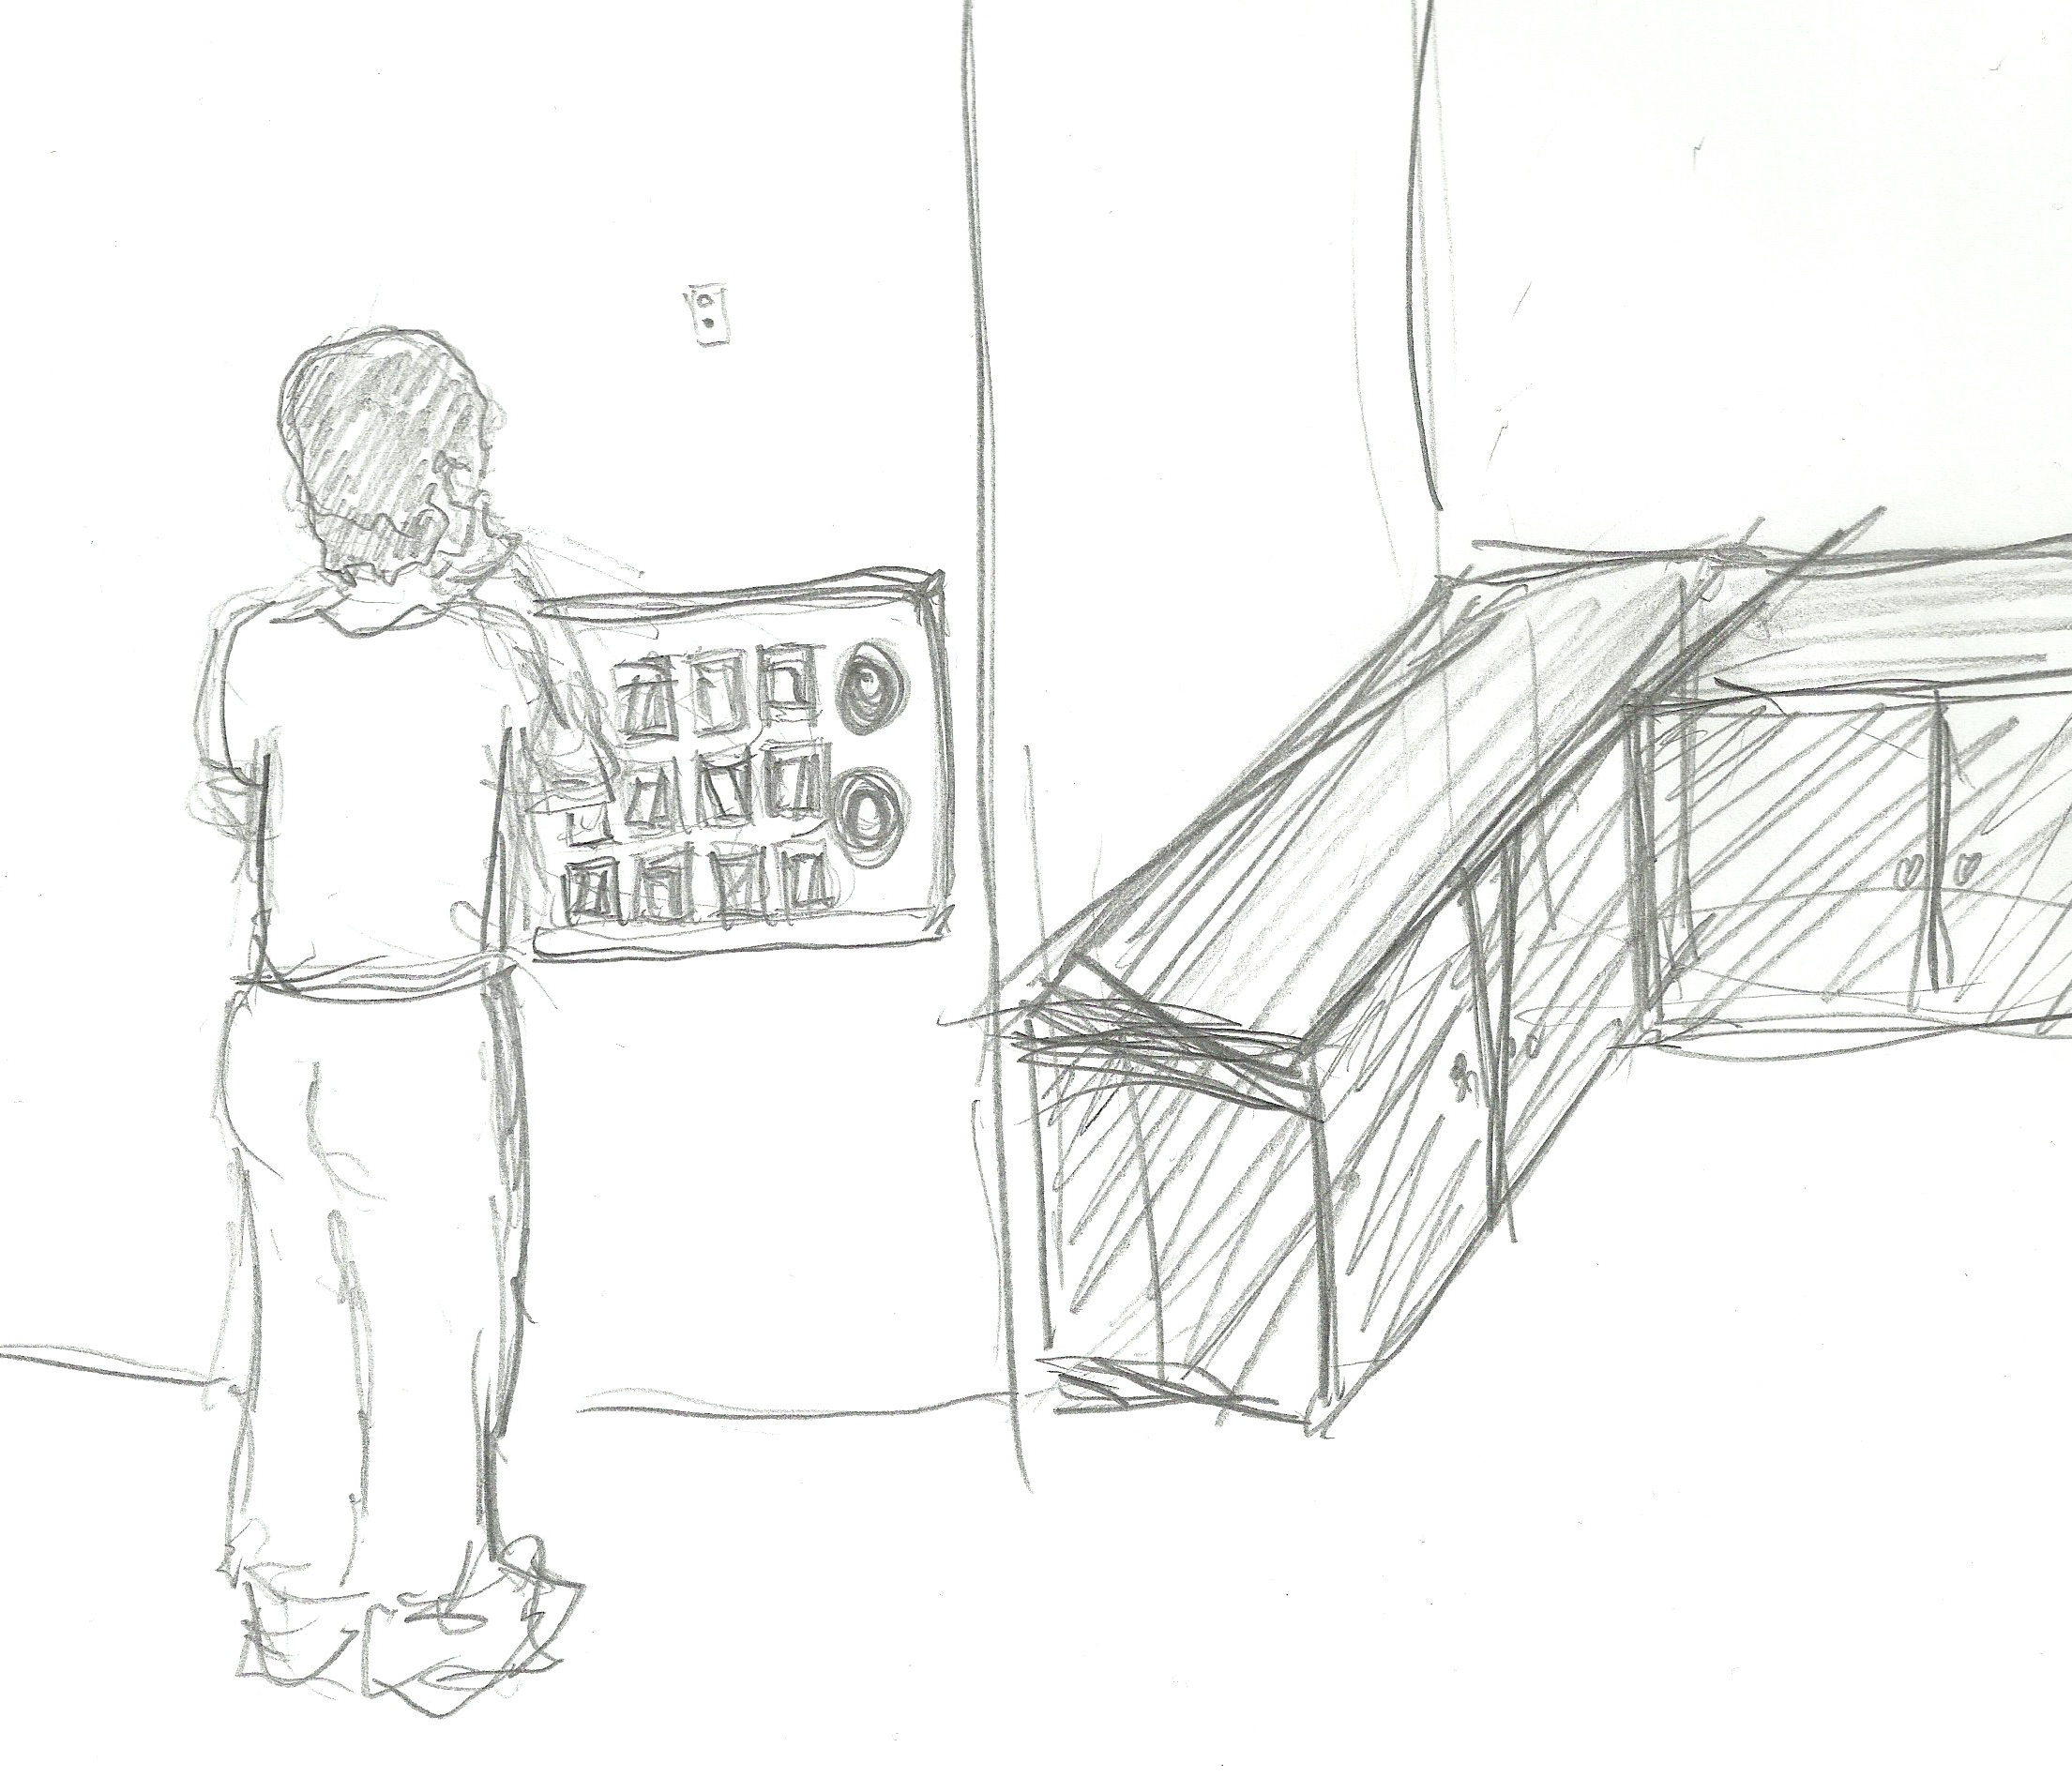
\includegraphics[scale=0.1]{fig/buttons}
\caption{En vegg med knapper skaper forvirring.}
\label{fig:panel}
\end{figure}
\subsubsection*{Hypotese 1}
\emph{En enkel sensor kan benyttes som en mekanisk bryter, og gjennom bruk av maskinlæring kan sensoren forstå et stort antall funksjoner.}

\subsubsection{Multimodal interaksjon gjennom tale og gester}
introduksjonstekst
\subsubsection*{Hypotese 2}
\emph{Kombinasjonen av enkle gester og begrenset tale er en tilstrekkelig, naturlig og effektiv måte å kontrollere hjemmet på. Det er er uproblematisk å implementere et slikt system med åpen kildekode.}

\subsubsection{Kombinasjoner}
introduksjonstekst
\subsubsection*{Hypotese 3}
\emph{Flere sensorer kan i kombinasjon benyttes til å oppnå enda større presisjon og fleksibilitet. Sensorene kan også utnyttes på alternative måter for å tilby ulik og forbedret interaksjon.}

\subsubsection{Kontekstdrevet brukergrensesnitt}
introduksjonstekst
\subsubsection*{Hypotese 4}
\emph{For å best mulig tilby brukere et brukergrensesnitt for det smarte hjemmet bør systemet være drevet av kontekst, ikke interaksjon.}




\subsection{Design av eksperimenter}
\subsubsection{Gestegjenkjennelse gjennom fotodioder}
{\color{red}Hvordan kan hypotesen testes?}

\subsubsection{Multimodal interaksjon gjennom tale og gester}
{\color{red}Hvordan kan hypotesen testes?}

\subsubsection{Kombinasjoner}
{\color{red}Hvordan kan hypotesen testes?}

\subsubsection{Kontekstdrevet brukergrensesnitt}
{\color{red}Hvordan kan hypotesen testes?}





\subsection{Implementasjon}
\subsubsection{Gestegjenkjennelse gjennom fotodioder}
{\color{red}Hvordan kan eksperimentet implementeres? Hvordan ble det implementert?}



Dette kapittelet har følgende bidrag:
\begin{itemize}
\item Jeg argumenterer for at en gestesensor i form av enkle fotodioder er et tilstrekkelig medium for enkel brukerinteraksjon (\ref{ch:2.minide}).
\item Jeg viser at maskinlæring kan benyttes for å lære et system å forstå enkle gester og viser at dette er et alternativ til å eksplisitt programmere forståelse (\ref{ch:2.resultater}).
\item Jeg viser at det holder med et titalls treningseksempler fra hver gest for å oppnå gode resultater med lineære modeller og at det med 50 eksempler oppnås en suksessrate på 96\% (\ref{ch:2.resultater}).
\end{itemize}

{\color{red}PING: Maskinlæring kan benyttes for å gi enkle sensorer en svært god forståelse av gester.}
Dette avsnittet presenterer hovedidéen for dette kapitellet. 
Dersom man ønsker å tilby styringsmuligheter på en eller flere vegger i et hus kan enkle gestesensorer benyttes i steden for et panel av knapper og dimmere. Selve sensoren er på størrelse med et knappenålshode og vi kan dermed forestille oss at designere kan komme opp med produktimplementasjoner som enten forsvinner inn i hjemmiljøet eller synes tydelig, men er praktisk og estetisk veldesignet. Sensoren merker at en hånd eller et annet objekt befinner seg foran den ved å sende ut et svakt infrarødt signal som reflekteres og detekteres dersom signalet er sterkt nok når det returnerer. Dette vil bare skje dersom objektet er opptil 20 cm unna sensoren. Dette betyr at gester kun forstås dersom de utføres rett foran sensoren. I motsetning til forståelse av gester gjennom bruk av kameraer er dette altså en langt mindre påtrengende måte å "lytte" etter innspill fra brukerne. Brukere kan være sikre på at de hverken overvåkes eller at personvernet deres på noen måte brytes. En slik gestesensor fungerer rett og slett kun som en multifunksjonell knapp.

\begin{wrapfigure}{r}{0.4\textwidth}
    \vspace{-20pt}
  \begin{center}
    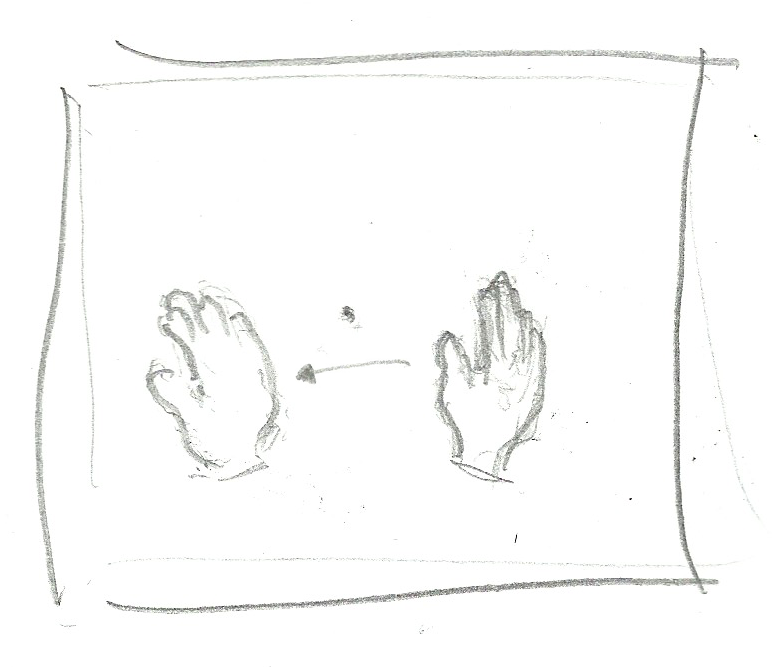
\includegraphics[width=0.35\textwidth]{fig/swipe-l-r}
  \end{center}
  \vspace{-20pt}
  \caption{Illustrasjon av en typisk gest.}
  \label{fig:gest}
  \vspace{-7pt}
\end{wrapfigure}

Figur \ref{fig:gest} viser en typisk gest der brukeren sveiper hånda foran sensoren som befinner seg på veggen. Vi kan forestille oss at denne sveipende bevegelsen foran denne sensoren betyr å skru av lyset i rommet sensoren befinner seg i. Men kanskje gesten betyr å skru på radioen, lukke gardinene eller starte kaffemaskinen. Det er ingen begrensning på hva en enkelt gest aktiverer i form av funksjonalitet.

Når en gest utføres må enten rådataene fra sensoren eller en forståelse av dataene sendes til en maskin som har ansvaret for å styre apparatene i hjemmet. Sensoren må være knyttet til en mikrokontroller eller tilsvarende som har ansvaret for å sende dataene videre. Dette kan enten være gjennom kabel eller trådløst. Det er mulig å programmere en mikrokontroller til å skille mellom sensordataene og forstå seks ulike gester {\color{red} ref}. Dette er i seg selv bra og betyr at en enkelt sensor kan fungere som en multifunksjonell knapp med minimum seks forskjellige kommandoer. Hvis man også utnytter at kombinasjonen av flere gester etter hverandre kan bety egne kommandoer er styringsmulighetene mange. Det finnes et alternativ til å programmere inn hva de ulike dataene skal tolkes som. Alternativet er å sende rådataene til en kraftigere maskin som kan benytte den spennende teknikken kjent som maskinlæring til å forstå enda flere ulike gester, med god sannsynlighet for suksess.

Maskinlæring handler om å la maskinen lære fra data. Dette kan enten være et forsøk på å finne ukjente sammenhenger i dataene den mates med eller det kan være å lære seg sammenhenger mellom dataeksempler og etiketter/klasser. Det er dette sistnevnte scenariet vi er interessert i. Vi kan mate maskinen med data fra en gest og samtidig gi informasjon om at dataene maskinen akkurat fikk betyr "sveip til høyre". Dermed kan maskinen danne en kobling mellom dataene som kom inn da vi sveipet til høyre og etiketten "sveip til høyre". Med tilstrekkelig treningseksempler fra de ulike gestene skal maskinen kunne lære seg forskjellene mellom de ulike gestene. Dermed vil den være i stand til å gjette riktig på hvilken gest vi utfører ved en senere anledning. Prototypen jeg har utviklet er trent med 50 ulike dataeksempler på hver av de 10 ulike gestene.

\begin{figure}[h]
\begin{subfigure}{0.23\textwidth}
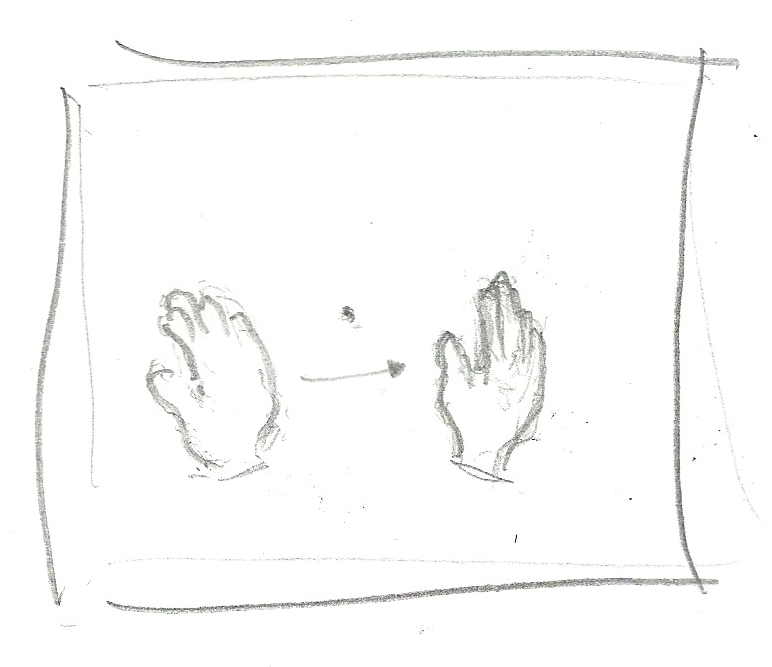
\includegraphics[width=3cm, height=3cm]{fig/swipe-r-l}
\caption{Sveip til høyre.}
\label{fig:sveip-}
\end{subfigure} 
\begin{subfigure}{0.23\textwidth}
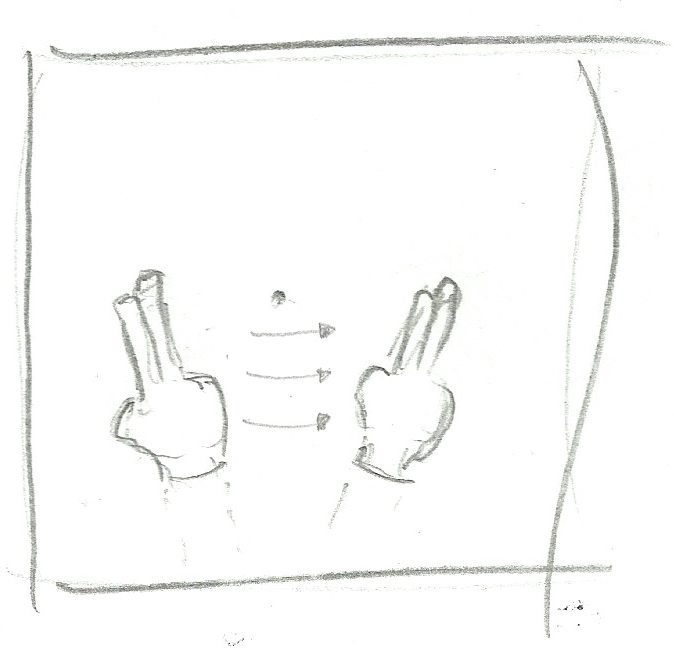
\includegraphics[width=3cm, height=3cm]{fig/flick-l-r} 
\caption{Flikk til høyre.}
\label{fig:flikk-h}
\end{subfigure}
\begin{subfigure}{0.23\textwidth}
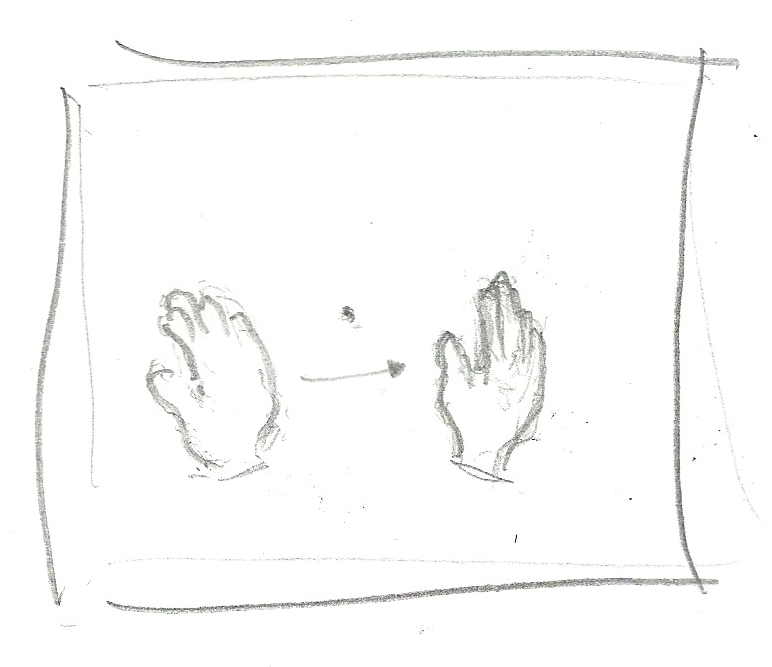
\includegraphics[width=3cm, height=3cm]{fig/swipe-r-l}
\caption{Sveip til venstre.}
\label{fig:sveip-v}
\end{subfigure} 
\begin{subfigure}{0.23\textwidth}
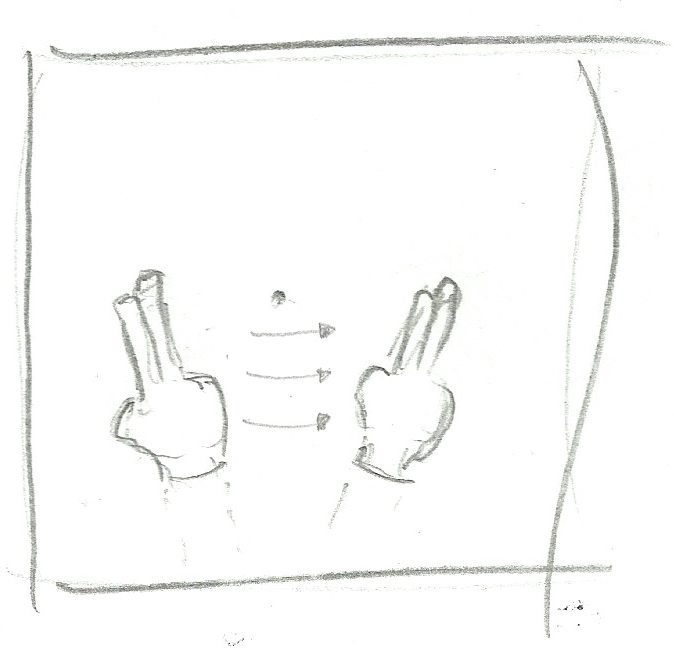
\includegraphics[width=3cm, height=3cm]{fig/flick-l-r}
\caption{Flikk til venstre.}
\label{fig:flikk-v}
\end{subfigure}
\begin{subfigure}{0.23\textwidth}
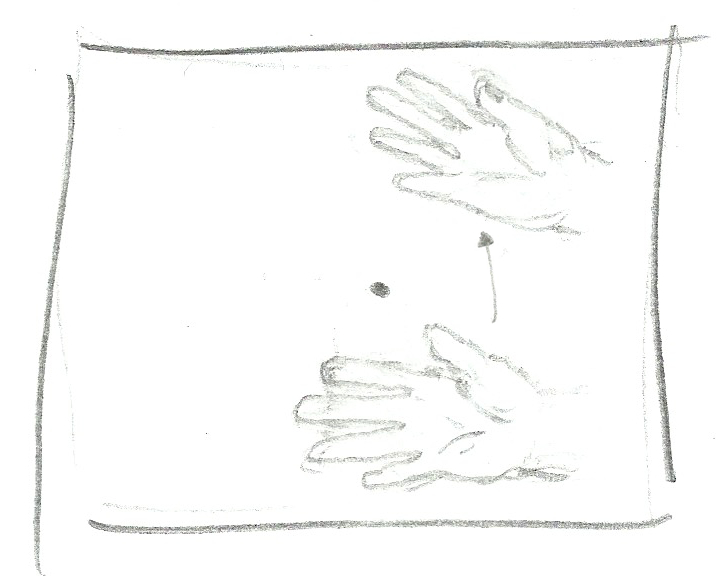
\includegraphics[width=3cm, height=3cm]{fig/swipe-d-u}
\caption{Sveip opp.}
\label{fig:sveip-opp}
\end{subfigure}
\begin{subfigure}{0.23\textwidth}
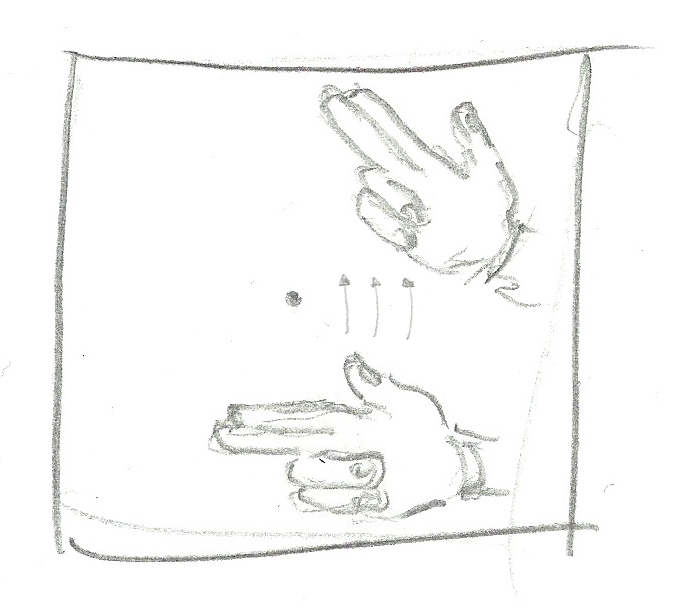
\includegraphics[width=3cm, height=3cm]{fig/flick-d-u}
\caption{Flikk opp.}
\label{fig:flikk-opp}
\end{subfigure}
\begin{subfigure}{0.23\textwidth}
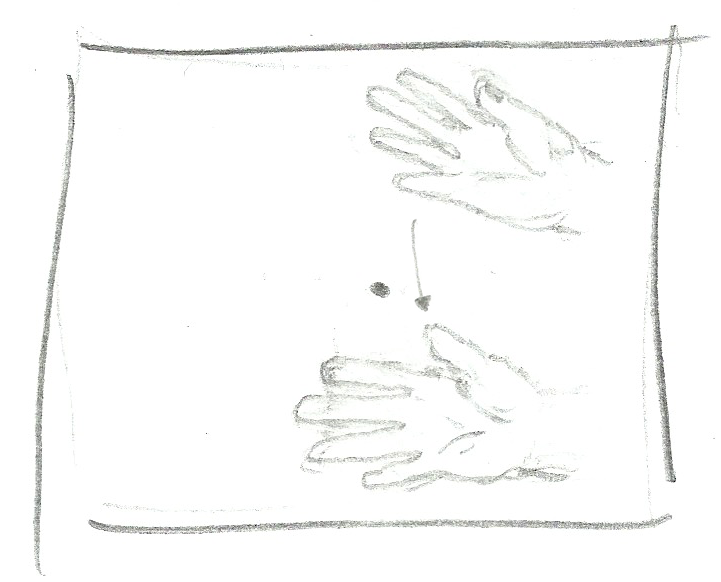
\includegraphics[width=3cm, height=3cm]{fig/swipe-u-d}
\caption{Sveip ned.}
\label{fig:sveip-ned}
\end{subfigure}
\begin{subfigure}{0.23\textwidth}
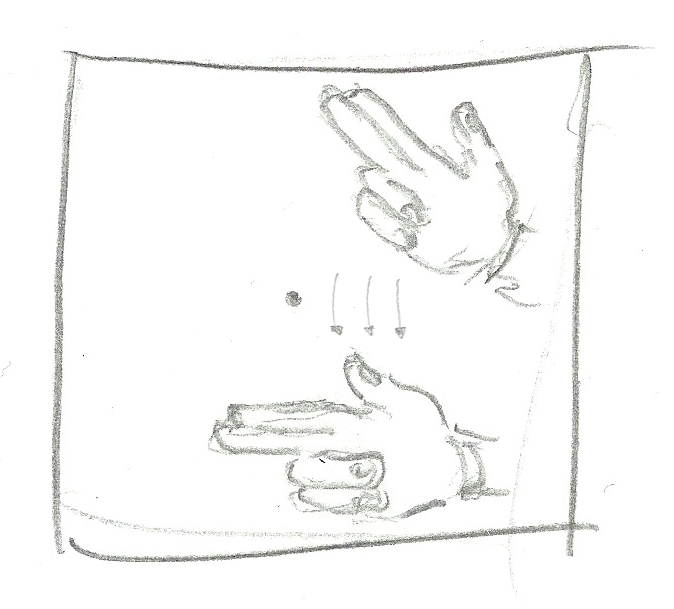
\includegraphics[width=3cm, height=3cm]{fig/flick-u-d}
\caption{Flikk ned.}
\label{fig:flikk-ned}
\end{subfigure}
\begin{subfigure}{0.25\textwidth}
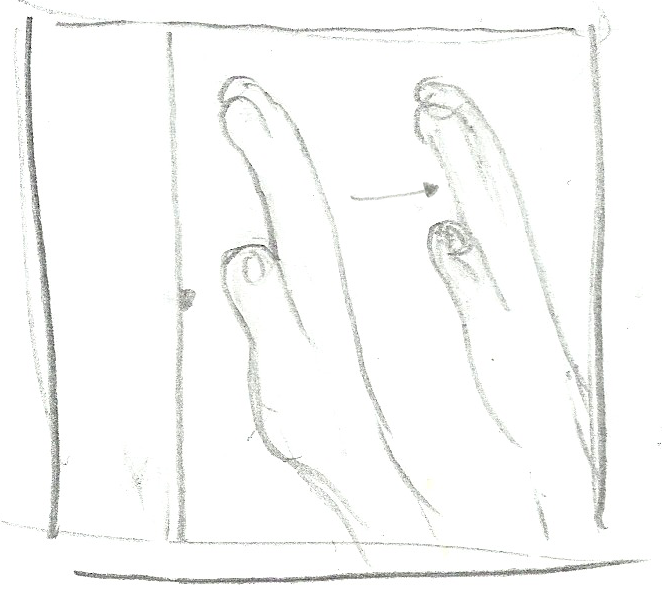
\includegraphics[width=3cm, height=3cm]{fig/near-far}
\caption{Nær - fjern.}
\label{fig:n-f}
\end{subfigure}
\begin{subfigure}{0.23\textwidth}
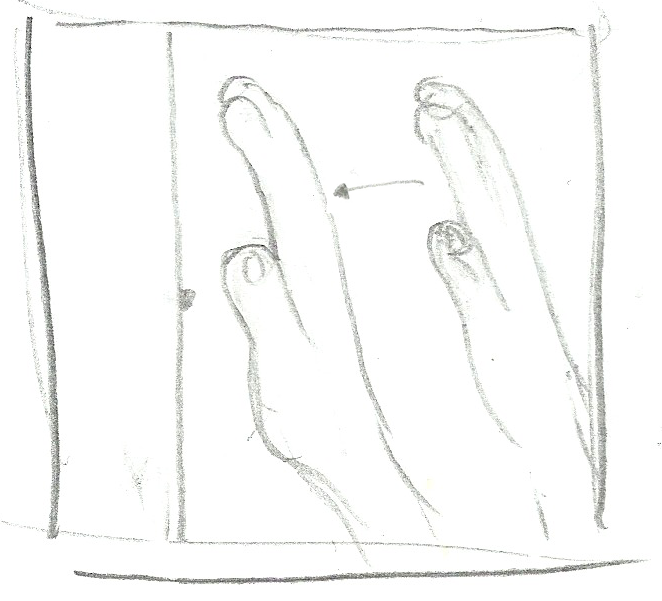
\includegraphics[width=3cm, height=3cm]{fig/far-near}
\caption{Fjern - nær.}
\label{fig:f-n}
\end{subfigure}
\caption{Illustrasjoner av de ulike gestene.}
\label{fig:gester}
\end{figure}

Sensoren som benyttes i denne prototypen er APDS-9960 fra Avago Technologies. Sensoren tilbyr måling av lys og farge, oppdagelse av nærhet og gestegjenkjennelse\footnote{Kapittel 4 utforsker bruksområder for funksjonaliteten rundt lys, farge og nærhet.}. Innpakningen er svært liten på kun 3.94 * 2.36 * 1.35 mm. Selve gestesensoren består av fire fotodioder som merker et reflektert infrarødt signal utsendt fra en LED. Fotodiodene er vinklet litt forskjellig slik at de plukker opp refleksjoner på litt forskjellige steder. Den benytter resultater fra nærhetsdetektoren for å automatisk aktiveres når et objekt er innen rekkevidde. I tilegg brukes måling av lys for å tilpasse de infrarøde målingene til lysnivået i omgivelsene. Dataene dannes som 32-bit datasett og kommuniseres over I2C-protokollen til en mikrokontroller. Gestesensoren kan selv håndtere forståelse av gester som passerer opp, ned, mot venstre eller mot høyre over sensoren, men denne funksjonaliteten tar vi ikke i bruk her {\color{red} ref apds9960-dokumentasjonen.}.

Prototypen er utviklet med Sparkfun's innpakning av APDS9960-sensoren\footnote{https://www.sparkfun.com/products/12787}. Denne brettet gjør APDS9960-sensoren tilgjengelig for enkel prototyping ved å bryte ut ulike pinner. {\color{red} bilde av sparkfun-brikken som peker ut hvilken del som er apds9960.} I tillegg har de gjort tilgjengelig programvare til Arduino-plattformen\footnote{http://www.arduino.cc/} så utviklere kommer raskt i gang. De ulike programmene som kan lastes opp til en Arduino gir tilgang til de forskjellige funksjonalitetene hos APDS-9960-brikken.

\subsubsection*{Dataprosessering}
Seriell data sendes fra mikrokontrolleren til datamaskinen som lytter på riktig port. Sensoren sender data så lenge ir-signalet reflekteres. Dette betyr at en gest som tar lengre tid skaper mer data. Et raskt flikk med to fingre skaper 16-32 datapunkter. Et rolig sveip over sensoren med hele hånda kan skape 100-200 datapunkter. En gest som involverer å holde hånda foran sensoren i et sekund eller mer skaper flere hundre datapunkter. Den variable mengden datapunkter skaper et problem; for å benytte de planlagte klassifiseringsteknikkene må hvert av treningseksemplene må ha like mange datapunkter.

Det finnes ulike metoder for å løse dette problemet. En av de er å bestemme et øvre antall maksimale datapunkter som skal tas med. Inputeksempler som ikke har tilstrekkelig med datapunkter blir paddet med 0-verdier. Å sette en maksgrense på datapunkter kan føre til at man mister viktig data fra gester som tar lengre tid å utføre. For et inputeksempel fra en rask gest vil mange datapunkter være 0. Dette kan påvirke effektiviteten til læringsalgoritmen. Et annet alternativ er å velge et fast antall datapunkter vært inputeksempel skal ha og så knytte inputeksempelet til denne vektoren av fast størrelse. Dersom inputdataene har få datapunkter blir vektoren sparsom, med dataverdiene spredt jevnt utover og med 0-verdier i mellom. Dersom inputdataene består av mange datapunkter vil hvert datapunkt i vektoren være et gjennomsnitt av en valgt mengde datapunkter.

Jeg valgte å benytte denne sistnevnte teknikken og lagde vektorer med 128 datapunkter. Dette tallet ble valgt basert på antall datapunkter som genereres ved ulike aktuelle gester. 128 datapunkter er nok til å gi tilstrekkelig detaljer selv ved gester som tar noe lengre tid og samtidig ikke så mange at raske gester skaper i overkant sparsomme vektorer. Vektoren normaliseres ved å knytte de mulige sensorverdiene [0,255] til [0,1.0]. Å illustrere dannelsen av vektorer med 128 datapunkter blir tungvint så i figur \ref{fig:data} har jeg illustrert prosessen med langt mindre data. I \ref{fig:few} består inputvektoren av to datapunkter. La oss si vi ønsker en vektor med størrelse fire og som er normalisert til verdiområdet [0,10.0]. Dette oppnås ved å spre inputdataene jevnt i vektoren og normalisere verdiene. \ref{fig:many} viser det motsatte tilfellet, der inputvektoren er for stor. For å representere dataene i en mindre vektor blir det tatt gjennomsnittsverdier som deretter normaliseres. 

\begin{figure}[h]
\centering
\begin{subfigure}{0.23\textwidth}
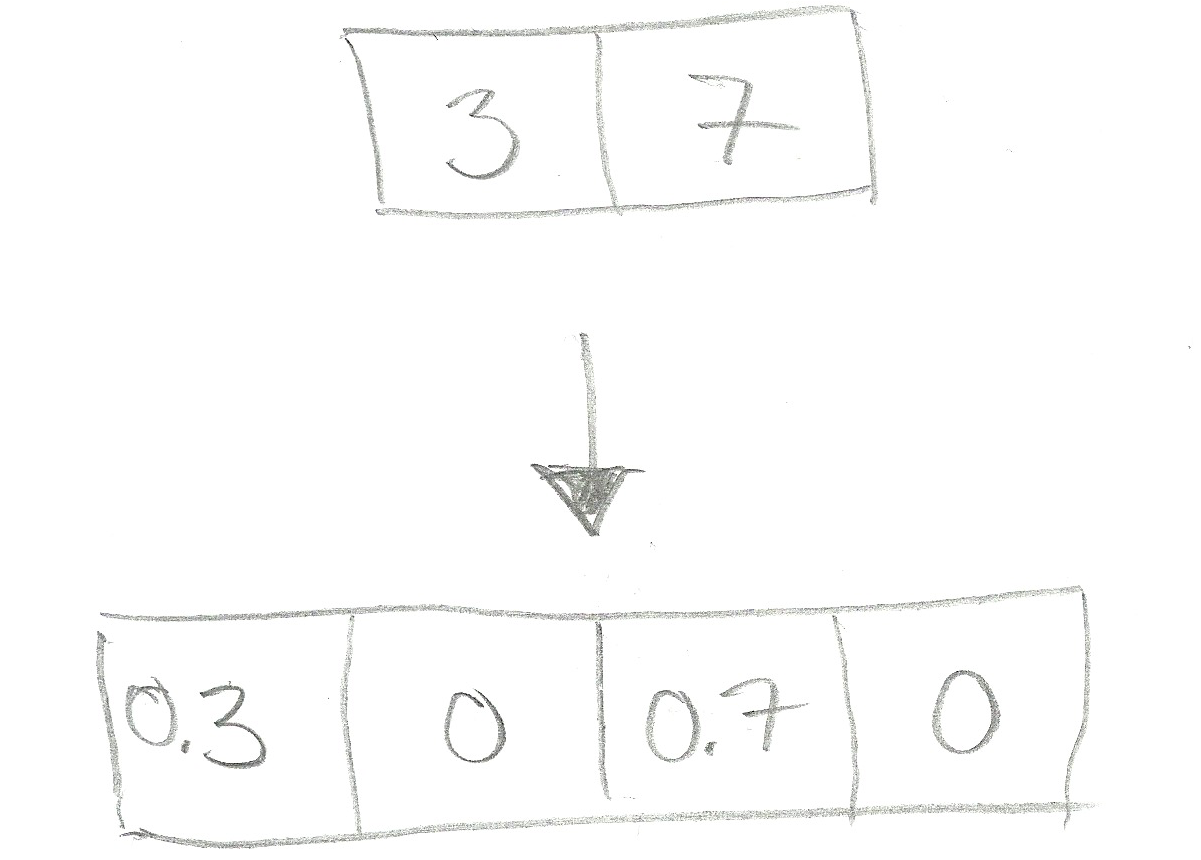
\includegraphics[width=3cm, height=3cm]{fig/few-to-many}
\caption{}
\label{fig:few}
\end{subfigure}
\begin{subfigure}{0.23\textwidth}
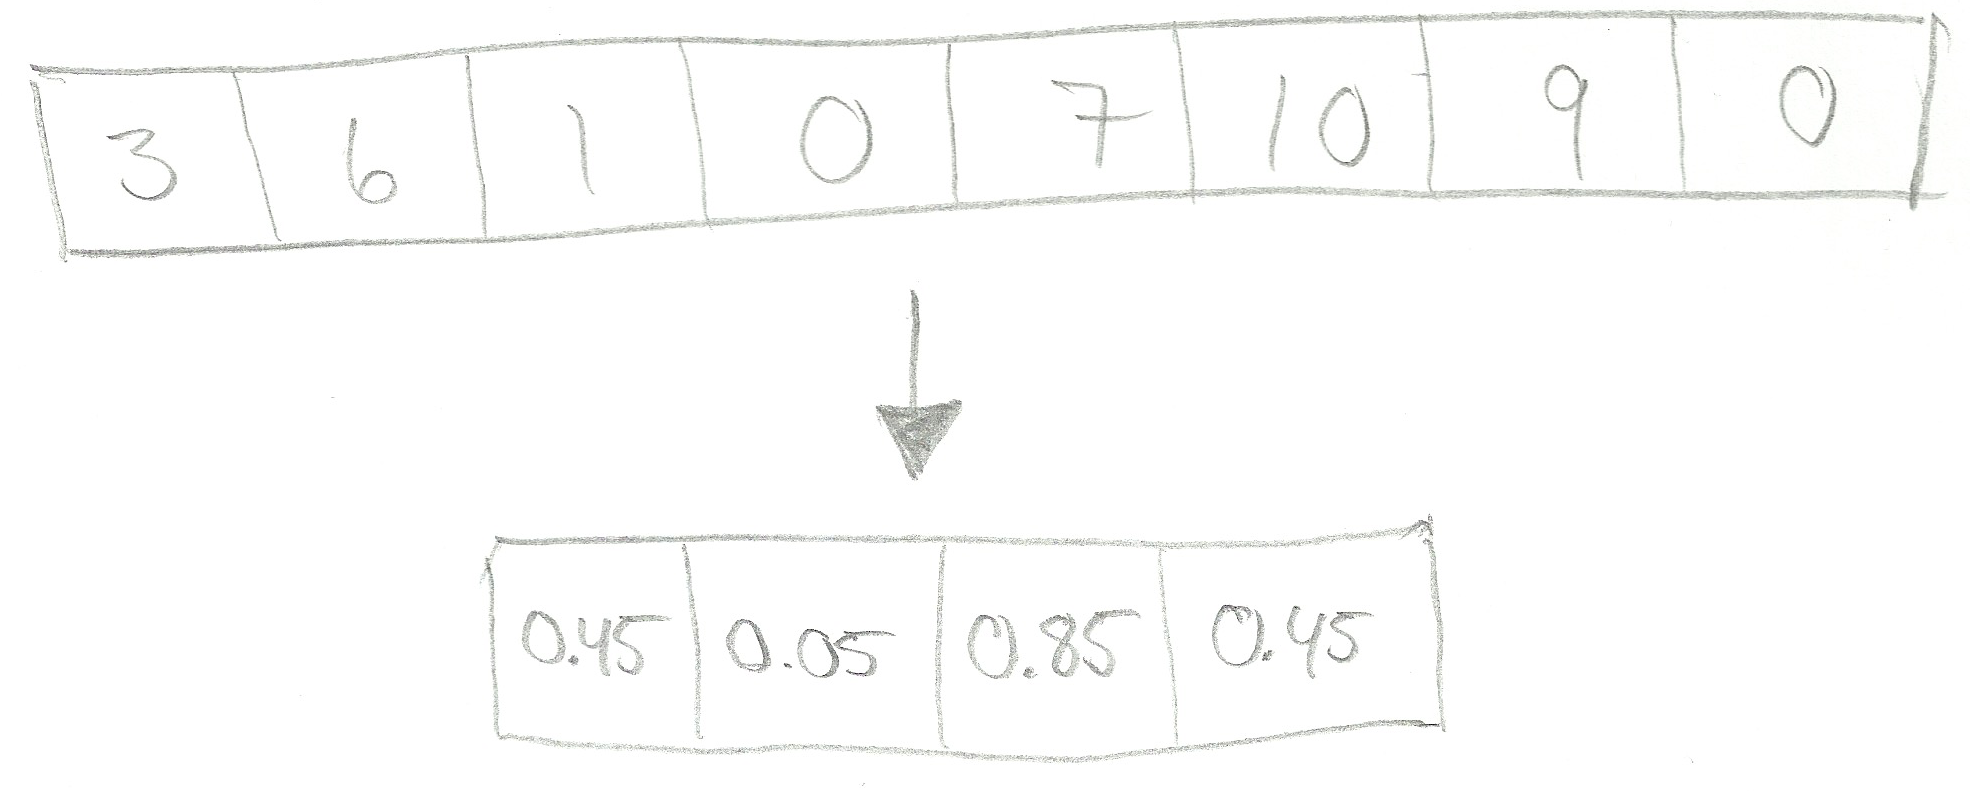
\includegraphics[width=3cm, height=3cm]{fig/many-to-few}
\caption{}
\label{fig:many}
\end{subfigure}
\caption{Illustrasjon av dannelsen av en egenskapsvektorer.}
\label{fig:data}
\end{figure}

{\color{red} ref process-data.py/trim-data}


\subsubsection{Multimodal interaksjon gjennom tale og gester}
{\color{red} Hvordan kan eksperimentet implementeres? Hvordan ble det implementert?}

Hva er en mer naturlig kommunikasjonsform enn tale? Generelt er det svært vanskelig å tenke seg andre former som kan beskrives som mer naturlige. Avhengig av hva som skal kommuniseres kan ulike tilnærminger være gode. Dersom man ønsker å skape noe gjennom manipulasjon blir tale raskt forbigått av en taktil kommunikasjonsform, som direkte kommunikasjon med hendene. Men når det gjelder å gi enkle kommandoer, å hente informasjon eller å kommunisere med andre mennesker kan tale fremstå som både den mest naturlige og effektive kommunikasjonsformen.

Drømmen om å kommunisere kontinuerlig med datamaskinen gjennom tale er tydelig gjennom både media og hvor penger til forskning plasseres. Denne oppgaven omhandler bruken av disse interaksjonsformene i konteksten av hjemmet. Så selv om tale kan være en interaksjonsform med stort potensiale i ulike domener må vi her spørre oss om å tilby tale som interaksjonsform er ønskelig i et hjem-scenario. 

{\color{red}PING: Kombinasjonen av enkle gester og begrenset tale er en aktuell og relativt enkelt implementerbar interaksjonsform for å styre det moderne hjemmet.}

Rejecting out of grammar utterances.


\subsubsection{Kombinasjoner}
{\color{red}Hvordan kan eksperimentet implementeres? Hvordan ble det implementert?}

Bruksområder i smarte hjem for den andre funksjonaliteten i sensorene.
PING: Data om farger, lysintensitet, avstand og en kombinasjon av flere gestesensorer utforskes for å finne nye interaksjonsideér.
Gester
Lysstyrke / Farger kontinuerlig
Lys interrupt
Nærhetsmåling kontinuerlig
Nærhetsinterrupt
Hva kan man få til dersom man har fire sensorer plassert i et kvadrat?

\subsubsection{Kontekstdrevet brukergrensesnitt}
{\color{red}Hvordan kan eksperimentet implementeres? Hvordan ble det implementert?}

{\color{blue}
Design av programvare

Design av programvare består av grafisk design (tegne bilder) og industriell design (tillate for mekanisk manipulasjon).

Informasjonsprogramvare er ikke en maskin, men et medium for visuell kommunikasjon.

Graphic design is the art of conveying a message on a two-dimensional surface. This is a broad field, because people have such a variety of messages to convey—identity, social status, emotion, persuasion, and so on. Most relevant to software is a branch that Edward Tufte calls information design—the use of pictures to express knowledge of interest to the reader.** Edward Tufte, The Visual Display of Quantitative Information (2001). Some products of conventional information graphic design include bus schedules, telephone books, newspapers, maps, and shopping catalogs. A good graphic designer understands how to arrange information on the page so the reader can ask and answer questions, make comparisons, and draw conclusions. When the software designer defines the visual representation of her program, when she describes the pictures that the user will interpret, she is doing graphic design, whether she realizes this or not.

Software is there to aid people
    To learn.
    To create.
    To communicate.

Informasjonsprogramvare er for å trene en intern modell. Manipulasjonsprogramvare er for å skape en ekstern modell. Kommunikasjonprogramvare er for å kommunisere en delt modell.

Information software serves the human urge to learn. A person uses information software to construct and manipulate a model that is internal to the mind—a mental representation of information. Good information software encourages the user to ask and answer questions, make comparisons, and draw conclusions. A person would use recipe software, for example, to decide what to cook for dinner. She would learn about various dishes (where “learning” could be as informal as a quick skim for something tasty that contains ingredients on hand), compare her options, and make her decision. In effect, she is constructing an internal understanding of culinary possibilities, and mentally prodding this model to reveal the optimal choice. It’s the same effect she would hope to achieve by consulting a recipe book.

Manipulation software serves the human urge to create. A person uses manipulation software to construct and manipulate a model external to herself—a virtual object represented within the computer, or a remote physical object. Some examples include software for drawing, writing, music composition, architectural design, engineering design, and robot control. Manipulation software can be considered a virtual tool—like a paintbrush or typewriter or bandsaw, it is used as an interface between creator and artifact.

Communication software serves the human urge to communicate. A person uses communication software to construct and manipulate an internal model that is shared with others—an understanding synchronized across multiple minds. Examples include software for email, group discussions (whether voice, video, or text), and collaborative working. In terms of raw mechanics, communication can be thought of as creating a response to information learned—that is, the external model manipulated by the speaker is the internal model learned by the listener. Thus, this paper will simply treat communication software as manipulation software and information software glued together, and mention it no further.** This dismissal is rather disingenuous—communication software is fundamentally unlike the other two because its user is a group, and a group as a whole can have different goals than any of its constituents individually. The considerations of social software design are well beyond the scope of this paper, but see Clay Shirky’s essays, particularly Social Software and the Politics of Groups (2003). This design approach is widespread—email software typically has separate reading and writing modes; messageboards similarly segregate browsing and posting.

Som regel når en person bruker programvare er det ikke for å skape noe, men for å lese, observere, utforske og lære. Folk er ute etter å ordne egne tanker. Datamaskinen er et medium for å spørre spørsmål, gjøre sammenligninger og dra konklusjoner.

Gjelder dette også for programvare i smarte hjem? Hva vil folk bruke det smarte hjemmet til?

Mye av dagens programvare møter disse behovene ved å presentere metaforiske objekter som skal manipuleres, men er dette egentlig nødvendig? Brukerne bryr seg ikke om disse kunstige objektene. De bryr seg om å se informasjonen og forstå valgene de kan ta. Modellen som skal manipuleres befinner seg i hodene deres.

A well-designed information graphic can almost compel the viewer to ask and answer questions, make comparisons, and draw conclusions. It does so by exploiting the capabilities of the human eye: instantaneous and effortless movement, high bandwidth and capacity for parallel processing, intrinsic pattern recognition and correlation, a macro/micro duality that can skim a whole page or focus on the tiniest detail. Meanwhile, a graphic sidesteps human shortcomings: the one-dimensional, uncontrollable auditory system, the relatively sluggish motor system, the mind’s limited capacity to comprehend hidden mechanisms. A graphic presents no mechanisms to comprehend or manipulate—it plugs directly into the mind’s spatial reasoning centers.

Eksempler rundt noe programvare som finnes i dag, spesielt for smarte hjem.

Design av programvare for informasjon burde tilnærmes som grafisk design. Utseende og hvordan informasjon presenteres bør være i fokus. Hva er den relevante informasjonen? Hva vil brukeren vite? Hvordan kan data vises på den mest effektiv måten? Hvordan kan teknikker fra grafisk design anvendes for å lede brukerens blikk mot løsningen? Brukeren bruker programvaren for å lære og han lærer ved å se på programvaren.

Hva slags funksjonalitet skal programvaren ha? Å klikke på en lysbryter bør naturligvis skru av eller på lyset. Å klikke på et kjøleskap eller vaskemaskin bør enten skru av og på eller gi mer informasjon om disse apparatene.

Edward Tufte's første regel for statistisk grafisk design: "vis dataene".

Spørsmål brukeren har om det smarte hjemmet sitt:

    What movies are showing today, at which times?
    What movies are showing around a particular time?
    Where are they showing?
    What are they about?
    Are they good?

Hvordan kan disse spørsmålene best besvares?

This is not a list of search results—it is an information graphic. It is for learning.

Just as important as what data is shown is where it is shown. Unlike the words in a paragraph, the elements in a graphic can be deliberately placed to encourage spatial reasoning. Unfortunately, most software graphics are arranged to maximize aesthetics, not to bring out useful relationships in the data.

Kontekst

The modern computer system provides the first visual medium in history to overcome this restriction. Software can:

    infer the context in which its data is needed,
    winnow the data to exclude the irrelevant, and
    generate a graphic which directly addresses the present needs.

Liberating us from the permanence of publication is the undersung crux of the computer—the dynamic display screen. Its pixels are magic ink—capable of absorbing their context and reflecting a unique story for every reader. And the components surrounding the display—CPU, storage, network, input devices—are its peripherals for inferring context.

Design av informasjonsprogramvare er design av kontekst-sensitiv informasjonsgrafikk.

All information software consists of context-sensitive graphics, whether the designer realizes it or not. For example, the list of query results from an internet search engine is a context-sensitive information graphic. The software’s data space consists of all the websites in the world. This is winnowed down to a dozen, using context that is inferred entirely from the search term contributed by the user. Clicking a “next” button contributes further context—dissatisfaction with the first set of results. Despite its enormous data space, this software restricts itself to a meager scrap of context, impersonal and imprecise.

There are, in fact, three sources from which software can infer context:

    Environment involves sensing the current state of the world.
    History involves remembering the past.
    Interaction involves soliciting input from the user.

Kontekst fra miljøet

Date and time. Time is one of the fundamental dimensions along which we organize our lives, and in any data space with a temporal dimension, “now” is almost always the prime landmark. Because users often seek information on demand, information related to “now” or “soon” is often the most relevant. Fortunately, every general-purpose computer knows when “now” is. A person using a software bus schedule, for example, should never have to hunt for the next bus.

Geographical location. Similarly, the most interesting spatial landmark is usually “here.” Unfortunately, this currently can be harder to determine automatically, but the payoff is enormous.** I believe that location is such vital context, Powerbooks should come with GPS receivers pre-installed, with an easy software API. Developers would then write software to take advantage of it, and other computer makers would follow suit. Someday, a computer without GPS might seem as silly as a computer without a clock. Obviously, a software roadmap needs to know the user’s location, but so does the bus schedule, as well as business listings, transportation planners, travel guides, and much other information software.

Physical environment. Given a time and location, many details of the physical environment, such as the weather, are just a network connection away. Consider a travel guide that suggests parks when sunny and museums when rainy.

Other information software, such as open websites. By reading some information, the user is indicating a topic of interest. All other information software should take heed. Consider a person reading the website of an upcoming stage play. When she opens her calendar, the available showings should be marked. When she opens a map, she should see directions to the playhouse. When she opens a restaurant guide, she should see listings nearby, and unless the play offers matinees, they shouldn’t be lunch joints.

Documents created with manipulation software. Creating some information indicates an even stronger topic of interest. Consider a person who requests information about “cats” while writing a paper. If the paper’s title is “Types and Treatment of Animal Cancer,” the information should skew toward feline medical data. The title “History of Egypt” indicates interest in ancient feline worship instead. And if the paper contains terms related to building construction, “cats” probably refers to the decidedly non-feline Caterpillar heavy machinery.

Email. Names, addresses, and phone numbers in recent email clearly constitute valuable hints. A recipient who opens a calendar should find the sender’s schedule juxtaposed with her own. When she opens a map, addresses in the email should be marked. But beyond that, recent correspondence can indicate current activities, and an email archive as a whole can describe the user’s characteristics and interests. Consider a person who requests information about “racing.” The fields of running, bicycles, and cars have distinct sets of terminology; if one set regularly shows up in the person’s conversations, “racing” isn’t so ambiguous.

A human doesn’t just use her senses to recognize her situation; she also uses memories of past situations. Software, too, can use its memory to understand the present. The current context, or a good approximation, can often be predicted from a history of past environments and interactions.

Last-value predictors represent the simplest form of prediction. They simply predict the current context to be the same as the previous one. This is reasonable in many situations where the user’s context is fairly static, changing slowly over the short term. For example, if yesterday, the user looked for one-bedroom apartments in North Berkeley, she is is probably still interested in one-bedroom apartments in North Berkeley today. If nothing else, the software should present this information immediately, without asking for details.

Last-value prediction is frequently thought of and implemented as manipulation of explicit state—that is, the context is a persistent object that remains as is unless changed by the user, so the software always appears as the user left it.** The engineering challenge then becomes merely persisting across invocations of the program. Often, not even this is bothered with. This stateful conceptual model mimics physical reality, and can be comfortable if the user cares enough about the software’s state to keep her own mental state in sync. However, this is often not the case with information software, especially software that is consulted intermittently. (If you put down a newspaper for a few hours, you won’t be distressed to find it on a different page when you return. You probably won’t even notice. On the other hand, you would be delighted if you often came back to find it on exactly the page you wanted to read.) By thinking of this as context prediction instead of state maintenance, the door is opened to more sophisticated predictors.

Learning predictors attempt a deeper understanding of the user. They construct a model to explain past contexts, and use the inferred relationships to predict the current context.

One simple approach to learning is to discover a common attribute of recent contexts, and narrow the current context along that attribute’s dimension. For example, in a music library, as the user chooses several bluegrass songs in a row, the software can graphically emphasize other songs in this genre. With further confidence, it might consider de-emphasizing or omitting songs outside of the genre. As another example, consider a user who requests information about “Lightwave,” then about “Bryce,” then “Blender.” These terms have many meanings individually, but as a group they are clearly names of 3D rendering software packages. A subsequent search for “Maya,” another 3D package, should not display information about the ancient civilization. In fact, information about Maya could be presented automatically.

Another simple approach is to establish the user’s velocity through the data space. If a person asks a travel guide about the Grand Canyon on one day, and Las Vegas the next day, the following day the software might suggest attractions around Los Angeles.** A better travel guide would suggest skipping Los Angeles.

In general, the problem is one of inferring a pattern that explains the user’s interests as a function of the environment, and extrapolating along the pattern to classify the current environment. As an example of general pattern modeling, consider a person who, as a byproduct of traveling to work, always checks the train schedule from Berkeley to San Francisco in the morning, and San Francisco to Berkeley in the evening. If the software can discover and model this pattern, it can present the appropriate information at each time without the user having to request it. When she looks in the morning, she sees by default the San Francisco-bound schedule; in the evening, the Berkeley-bound schedule. Again, this may sound daunting to an engineer. Implementation will be discussed later in the paper.

Large histories can enable some very sophisticated predictors, especially if it is possible to reach into the environment and correlate with other users’ histories. For example, by asking their users to rate each movie they return, Netflix is able to infer some enormously valuable context—each user’s taste. This allows them to winnow an enormous dataset (their catalog of movies) down to a dozen data points (movies the user hasn’t seen, which were enjoyed by people with similar taste), which can be presented in a single, navigation-free graphic. The winnowing is impressively on-target—two-thirds of users’ selections come from recommendations.** Laurie J. Flynn, Like This? You’ll Hate That. New York Times, Jan. 23, 2006. TiVo similarly uses a collaborative predictor to infer which television programs the user would be interested in. These are presented on a “suggestions” page, and recorded automatically when possible.** For technical details, see Ali and van Stam’s paper TiVo: Making Show Recommendations Using a Distributed Collaborative Filtering Architecture (2004).

Amazon, iTunes, and an increasing number of other online retailers are currently incorporating similar schemes. However, with the exception of the lowly junk-mail filter, non-retail information software that learns from history is still rare. Typically, users can only hope for last-value prediction, if that. Most software wakes up each day with a fresh case of amnesia.

Unfortunately, software that doesn’t learn from history dooms users to repeat it. And repeat it they will—tediously explaining their context, mouse click by mouse click, keystroke by keystroke, wasted hour by wasted hour. This is called interactivity.

Chris Crawford defines interaction as a three-phase reciprocal process, isomorphic to a conversation: an interactant listens to her partner, thinks about what was said, and speaks a response. Her partner then does the same.** See Crawford’s book The Art of Interactive Design (2003), or his essay Fundamentals of Interactivity (1993). For manipulation software, interaction is perfectly suitable: the user views a visual representation of the model, considers what to manipulate next, and performs a manipulation. The software, in turn, inputs the user’s manipulation request, updates the model, and displays the updated representation. With good feedback and an effective means of “speaking” to the software, this process can cycle smoothly and rapidly. It mimics the experience of working with a physical tool.

Programvare for informasjon etterligner opplevelsen av å lese, ikke å jobbe. Det brukes for å oppnå en forståelse og for å konstruere en mental modell. Brukeren må altså lytte til programvaren og tenke på hva den sier. Enhver manipulering foregår i brukerens hode. Den eneste grunnen til å interagere er dermed å eksplisitt gi ekstra kontekstinformasjon som programvaren ikke selv kan finne ut av. Dette indikerer subsettet av informasjon som er relevant. For programvare for informasjon er interaksjon å navigere i dataene.

For programvare for informasjon er all interaksjon å spesifisere kontekst. Hver interaksjon bør resultere i en forståelig forandring i kontekst-sensitiv informasjonsgrafikk. Ved å gi direkte tilbakemelding reduserer mengden manipulasjon brukeren må utføre for å få et tilstrekkelig syn på dataene.

Interaction should be used judiciously and sparingly, only when the environment and history provide insufficient context to construct an acceptable graphic.

When the user is forced to interact, the software assumes the form of manipulation software. The external model, manipulated through navigation, is the software’s model of the context. However, unlike genuine manipulation software, the user does not care about this model—it is merely a means to the end of seeing relevant information.

Kontekst kan forstås fra brukerinteraksjon, men kun som en siste utvei. Den beste måten å minimere eller fjerne interaksjon er gjennom informasjonsrik grafisk design, som bruker miljøet og historie. Gjenværende interaksjon kan løses med grafisk manipulasjon, relativ navigasjon og en tett feedback-loop.

Graphical manipulation. Command-line systems are criticized for forcing the user to learn the computer’s language. Modern GUIs may be easier to use, but they are not much different in that respect. The GUI language consists of a grammar of menus, buttons, and checkboxes, each labeled with a vocabulary of generally decontextualized short phrases. The user “speaks” by selecting from a tiny, discrete vocabulary within an entirely fixed grammatical structure—a bizarre pidgin unlike any human language, unexpressive and unnatural.

Relative navigation. If the software properly infers as much as possible from history and the environment, it should be able to produce at least a reasonable starting point for the context model. Most of the user’s interaction will then consist of correcting (or confirming) the software’s predictions. This is generally less stressful than constructing the entire context from scratch.


For example, Google Maps offers both absolute navigation (typing in an address) and relative navigation (panning and zooming the current map). However, it initially displays by default the entire continent; this effectively demands that the user type in an absolute location to get started.** The user can manually specify an initial location, but she will presumably set this to her home. Ironically, her own neighborhood is the least likely place she’ll need mapped. A better design might start at the last place the user looked (last-value prediction), with a nearby list of locations predicted by history (recently visited or manually bookmarked) and the environment (addresses extracted from email, open websites, and calendar software). A reasonable starting point would almost always be a click away, and from there, the user could use relative navigation (dragging and zooming) or simply “navigate” by eye if the graphic is detailed enough. Conceptually, a prediction list might itself be considered relative navigation, as a set of “shortcuts” through the data space.


An even better design would recognize the prediction list as information software in its own right, and would take steps to show the data (such as annotating the predictions with driving times to and from common locations, taking current traffic conditions into account) and arrange the data (perhaps spatially arranging the predictions on their own map). This might answer most of the user’s questions without any interaction at all.

This principle is universal. If the user clicks a checkbox and nothing happens, her action is rendered ambiguous or even meaningless. She cannot evaluate a response and let it guide her next action. In terms of Crawford’s conversation metaphor, the software is failing to speak back—she is shouting into the wind.


For information software in particular, all interaction specifies context. Thus, each interaction can and should result in a discernible change to a context-sensitive information graphic. Providing immediate feedback reduces the amount of manipulation the user must do before either reaching an adequate view or recognizing a wrong turn and backtracking.


Any web form with a “submit” button or dialog box with an “accept” button fails this point. Google Maps offers reasonable feedback during relative navigation, but none during absolute navigation, such as typing in an address. Even a simple predictive auto-complete would be helpful, but consider the possibilities suggested by Ben Fry’s zipdecode applet. (First click “zoom” in the lower-right, then type in numbers.) Imagine honing in on familiar areas simply by typing the first few digits of a zip code—type “9” to immediately zoom into the US west coast, followed by “4” to zoom into the SF bay area and then “5” for the east bay. Because of the immediate feedback, the user can stop typing when she gets close enough, and use relative navigation from there.

The choice of graphical representation depends on what sort of data space is left after context-based winnowing. What context can be inferred?

Instead of having to name the station, the user effectively points at the map and says, “There!” Although it is less important in this case, the feedback loop remains tight; the train chart updates as the markers are moved.
 
Instead of the user continually asking “Should I start walking to the station now?”, she might prefer the software to notify her directly: “Start walking to the station now!” Audio works well for infrequent, asynchronous notifications. The widget can speak announcements of upcoming trains. 

A typical design would use a preference dialog or form that the user would manipulate to tell the software what to do. However, an information design approach starts with the converse—the software must explain to the user what it will do. It must graphically express the current configuration.

For presenting abstract, non-comparative information such as this, an excellent graphical element is simply a concise sentence.

As with the map, once the information graphic is established, manipulation can be incorporated. In this case, some words are colored red, and the user can click on these words to change them.

The user always sees the software presenting information, instead of herself instructing the software. If the information presented is wrong, the user corrects it in place. There is no “OK” or confirmation button—the sentence always represents the current configuration. The graphic fades out when the mouse is clicked outside of it or the mouse leaves the widget.

Ironically, the BART widget appears so fresh because its underlying ideas are so old. The time bar graph was invented about 250 years ago. The map and the written sentence are both about 5000 years old. They are beautiful, venerable forms of visual communication. The bugs have been worked out. They are universally, intuitively understood.

The pulldown menu, the checkbox, and the bureaucracy-inspired text entry form were invented 25 years ago, desperation devices to counter inadequate technology. They were created for a world that no longer exists.

Twenty-five years from now, no one will be clicking on drop-down menus, but everyone will still be pointing at maps and correcting each others’ sentences. It’s fundamental. Good information software reflects how humans, not computers, deal with information.

There is some attempt to use color symbolically. On the map, the calendar, and the flight chart, green represents “home,” and yellow the destination. However, it is not critical that the user notice this.

Last-value prediction (automatically selecting the last route purchased, and displaying a list of recent trips) may eliminate or reduce the map clicks for many travelers. A learning predictor, capable of inferring that the user always spends the first Monday through Friday of the month in Baltimore and selecting that range on the calendar automatically, could eliminate all context-establishing interaction, leaving only the decision-conveying interaction of clicking ticket prices. Of course, since everything is on the same page and feedback loops are tight, the user can explore different dates and cities, and see the available flights immediately.

The section “Inferring context from history” presented the need for software to learn from the past. Good information software will attempt to predict current context by discovering patterns in past contexts. Although such application software is rare, there is nothing novel or exotic about the algorithms required. The computer science discipline devoted to this subject is called “machine learning” or “learning systems,” and several decades of research have produced a variety of algorithms for modeling and predicting behavior.*

Consider the example presented earlier of a train trip planner that predicts the route that the user wants to see. There are typically daily or weekly patterns to a person’s local travel schedule. A planner that models these patterns could automatically present the user with appropriate information, eliminating most interaction.

History collection. Each time the user indicates interest in a particular route, it is recorded in a history with the date and time. The user indicates interest either by explicitly switching the planner to display a route, or by looking at the planner and then looking away, indicating that the shown route is still interesting.

Prediction. When the user looks at the planner, each history entry “votes” for its route with a certain weight, and the route with the largest total weight is displayed. Each entry’s weight is a product of three factors, which depend on the time, the day of the week, and the age of the history entry.

Time. If the time is 9:00, the user’s route at 9:10 yesterday is very relevant. What the user did at 10:00 is not quite so relevant, and her 12:00 activity is probably unrelated. Thus, each vote is weighted by a window around the time of the history entry. Typically, if the user is preparing to catch a train, she won’t just look once at the planner and memorize the time. She will glance at the planner frequently over a span of time. Each of these looks should not count as an individual vote. Instead, the entire span of checking is coalesced into a single history entry, with a widened time window. (Also, throughout these frequent check-ups, the user sees only last-value prediction. Learning prediction is only used if some time has passed since the previous look.)

Day of the week. A user will typically exhibit a superposition of daily patterns, such as going to and from work, and weekly patterns, such as cello practice every Tuesday. To allow for both, history entries from a different weekday are allowed to vote, but have a smaller weight. The bleed across days allows the algorithm to learn daily patterns faster, but because other days are penalized, weekly patterns can be learned as well. Saturday and Sunday are independent from weekdays and from each other.

Age. Older history entries are given less weight, and eventually are forgotten. This makes the algorithm adaptive. If the user adopts a new pattern, such as switching jobs or joining the Thursday-night knitting circle, the algorithm is able to keep up, instead of having to be manually reset.

The section “Inferring context from the environment” presented a number of environmental sources from which information software could infer context. The hardware-related sources, such as clocks and location sensors, might have seemed obvious. The software-related sources, such as other information software and documents created with manipulation software, might have seemed so far-fetched as to be implausible. This section will present the information ecosystem, a software architecture which might allow for such behavior.

}